\documentclass[tikz,border=10pt]{standalone}
\usetikzlibrary{shapes.geometric, shapes.symbols, arrows.meta, positioning, calc, fit, backgrounds}

\begin{document}
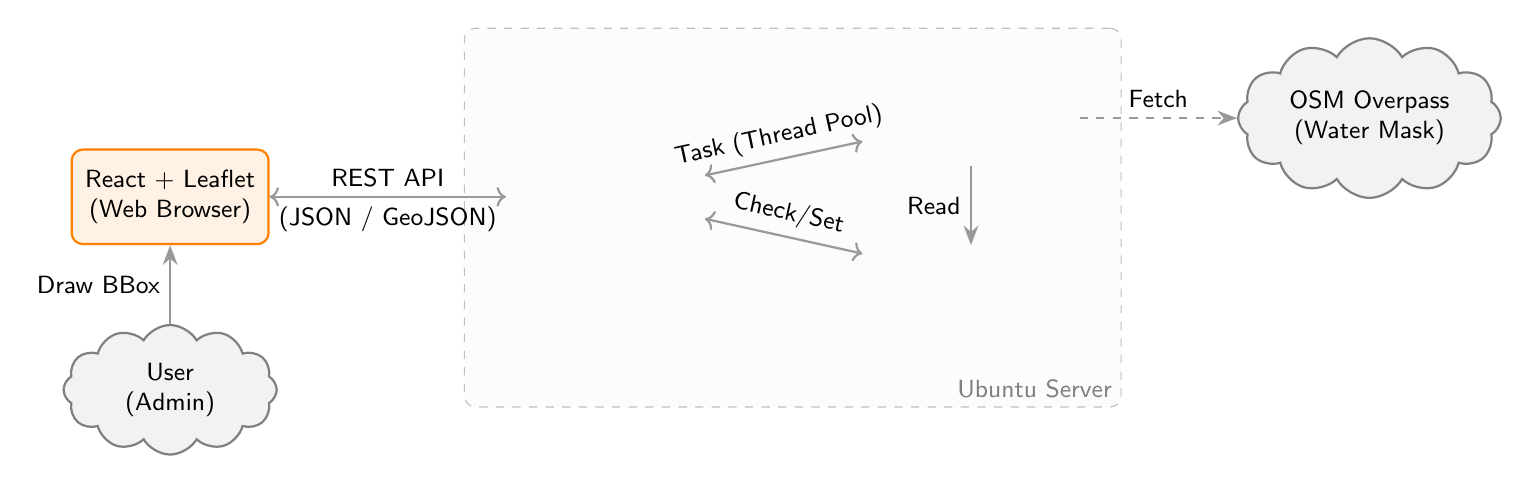
\begin{tikzpicture}[
    auto,
    node distance = 1.5cm and 2cm,
    font=\sffamily\small,
    box/.style = {rectangle, draw=blue!60, fill=blue!5, thick, rounded corners, minimum height=1.2cm, minimum width=2.5cm, align=center},
    db/.style = {cylinder, draw=black!60, fill=gray!10, shape border rotate=90, aspect=0.25, thick, minimum height=1.5cm, minimum width=2.5cm, align=center},
    ext/.style = {cloud, draw=gray, fill=gray!10, cloud puffs=12, cloud puff arc=120, aspect=2, thick, align=center},
    arr/.style = {-{Stealth[length=2.5mm]}, thick, draw=gray!80},
    group/.style = {rectangle, draw=gray!50, dashed, inner sep=15pt, fill=gray!2, rounded corners}
]

    % Frontend
    \node [box, fill=orange!10, draw=orange] (browser) {React + Leaflet\\(Web Browser)};
    
    % Backend Group
    \begin{scope}[local bounding box=backend]
        \node [box, fill=green!10, draw=green!70!black, right=3cm of browser] (fastapi) {FastAPI Server\\(Port 5000)};
        \node [box, right=2cm of fastapi, yshift=1cm] (geo) {Geo Pipeline\\(pysheds, rasterio)};
        \node [box, right=2cm of fastapi, yshift=-1cm] (cache) {Redis Cache\\(Port 6379)};
        \node [db, below=1cm of geo] (srtm) {Local SRTM\\HGT Tiles};
    \end{scope}
    
    \node[group, fit=(fastapi) (geo) (cache) (srtm)] (backend_box) {};
    \node[anchor=south east] at (backend_box.south east) {\color{gray}Ubuntu Server};

    % External
    \node [ext, right=2cm of geo] (osm) {OSM Overpass\\(Water Mask)};
    \node [ext, below=1cm of browser] (user) {User\\(Admin)};

    % Edges
    \draw [arr] (user) -- node[left] {Draw BBox} (browser);
    \draw [arr, <->] (browser) -- node[above] {REST API} node[below] {(JSON / GeoJSON)} (fastapi);
    \draw [arr, <->] (fastapi) -- node[above, sloped] {Check/Set} (cache);
    \draw [arr, <->] (fastapi) -- node[above, sloped] {Task (Thread Pool)} (geo);
    \draw [arr] (geo) -- node[left] {Read} (srtm);
    \draw [arr, dashed] (geo) -- node[above] {Fetch} (osm);

\end{tikzpicture}
\end{document}
